\documentclass[runningheads]{llncs}
\usepackage{amsmath,amssymb}
\usepackage{graphicx}
\usepackage{booktabs}
\usepackage{multirow}
\usepackage{url}
\usepackage{hyperref}
\usepackage{xcolor}

\begin{document}

\title{IntentAgent: Intent-Aware Progressive Intelligent Retrieval\\for Retrieval-Augmented Generation}

\author{Author Names}
\institute{Institute Names}

\maketitle

\begin{abstract}
The performance of Retrieval-Augmented Generation (RAG) systems depends critically on retrieval quality, yet existing methods apply a uniform retrieval strategy to all queries, neglecting the decisive influence of query intent diversity on retrieval path selection. This paper proposes IntentAgent, an intent-aware progressive intelligent retrieval method for RAG built on the principle that queries with distinct intent types should be directed to differentiated retrieval strategies and that this routing mechanism should progressively evolve from static rules to dynamic, adaptive decisions. IntentAgent comprises three progressive stages: (1)~six-class intent recognition through a dual-path classifier that combines an LLM with rule-based fallback, paired with static strategy routing; (2)~dynamic tool orchestration on a directed state graph, in which a reasoning-action protocol enables the LLM to autonomously select retrieval tools and a reflection loop enforces quality control; and (3)~experience memory augmentation via intent-bucketed persistent storage with a recall-inject-persist closed loop that enables cross-session self-improvement. Experiments on HotpotQA, 2WikiMultiHopQA, and MuSiQue demonstrate that IntentAgent outperforms existing text-based, graph-based, and hybrid retrieval methods on the majority of metrics under both Qwen3-8B and Qwen3-32B backbone models.

\noindent\textit{Keywords:} Retrieval-Augmented Generation, Intent Classification, Dynamic Retrieval Strategy, Experience Memory, Agent, Multi-hop Question Answering
\end{abstract}

\section{Introduction}

Retrieval-Augmented Generation (RAG) augments LLMs with external knowledge retrieval at inference time and has become the predominant paradigm for mitigating hallucinations and improving factual accuracy~\cite{ref1}. A typical RAG system follows a retrieve-read-generate pipeline: given a user query, relevant passages are first retrieved from a knowledge base and then supplied as context to the LLM for answer generation~\cite{ref2}.

Existing RAG systems, however, share an implicit and restrictive assumption at the retrieval stage, which we term the \emph{strategy homogeneity assumption}: regardless of query intent, the system applies the same retrieval pipeline---typically a single-pass vector similarity search. This assumption breaks down in the face of real-world query diversity. Consider three representative query types. A factual query such as ``Who invented the World Wide Web?'' requires only a single vector retrieval to locate the answer passage. A multi-hop reasoning query such as ``What influence did the alma mater of Einstein have on the development of quantum mechanics?'' demands bridging inference across multiple entities, and a single retrieval pass rarely covers the complete evidence chain. A comparative query such as ``Compare the performance of BERT and GPT on text classification tasks'' requires parallel retrieval of information about two entities followed by structured comparison.

The optimal retrieval paths for these three query types differ substantially. Routing a multi-hop reasoning query through a single-pass vector retrieval pipeline often yields incomplete or missing evidence, whereas applying a complex multi-hop strategy to a simple factual query introduces unnecessary latency and computational overhead.

\begin{figure*}[htbp]
\centering
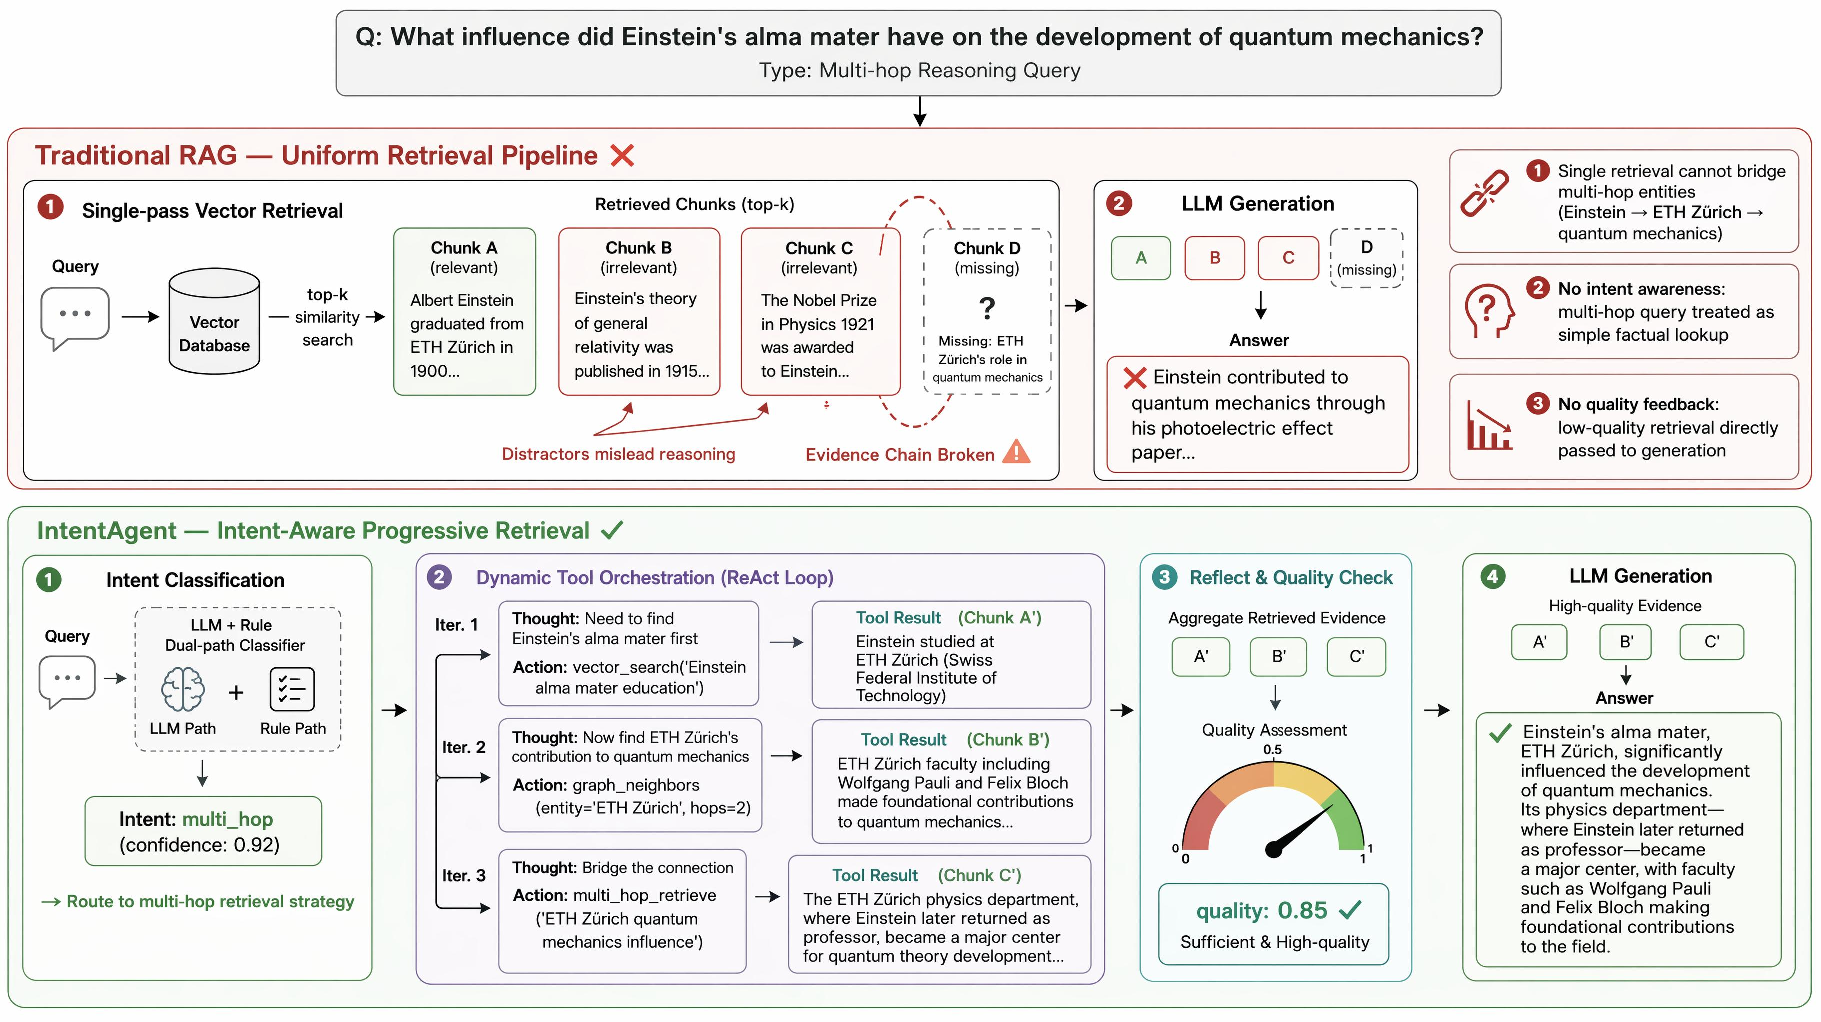
\includegraphics[width=\textwidth]{figures/figure1.pdf}
\caption{Comparison between conventional RAG and IntentAgent. Taking the multi-hop query ``What influence did the alma mater of Einstein have on the development of quantum mechanics?'' as an example, the upper half illustrates how conventional RAG suffers from evidence chain breakage and distractor interference due to strategy homogeneity, while the lower half shows how IntentAgent assembles the complete evidence chain through intent-aware progressive retrieval.}
\label{fig:comparison}
\end{figure*}

The central proposition of this paper is that query intent should serve as a first-class citizen in retrieval strategy selection. We instantiate this proposition as IntentAgent, whose design strikes a balance between controllability and adaptivity through three-stage progressive evolution.

In the first stage, static intent routing, we define a taxonomy of six query intent classes (factual, analytical, comparative, multi\_hop, exploratory, and follow\_up) and design a dual-path classifier that cascades an LLM with rule-based fallback. Classification results are routed to predefined retrieval strategies via a deterministic mapping table.

In the second stage, dynamic tool orchestration, we address the inability of static routing to handle cross-intent queries and runtime adaptation. A directed state graph restructures the retrieval process as an LLM-driven tool selection loop: the LLM autonomously decides which retrieval tools to invoke and in what order following a reasoning-action protocol~\cite{ref13}, while a reflection node evaluates evidence quality and triggers replanning when the quality score falls below a threshold.

In the third stage, experience memory augmentation, we address the limitation that dynamic orchestration starts every decision from scratch. Intent-bucketed persistent experience storage implements a recall-inject-persist closed loop, giving the system cross-session self-improvement capability.

We conduct systematic experiments on HotpotQA~\cite{ref20}, 2WikiMultiHopQA~\cite{ref21}, and MuSiQue~\cite{ref22} under both Qwen3-8B and Qwen3-32B backbone models. Results demonstrate that IntentAgent achieves the best or highly competitive performance against all representative baselines, including Vanilla RAG, RAPTOR~\cite{ref23}, TOG~\cite{ref24}, G-Retriever~\cite{ref25}, LightRAG~\cite{ref26}, GraphRAG~\cite{ref27}, and HippoRAG~\cite{ref28}, across all datasets and backbone configurations.

The main contributions of this paper are as follows. (1)~We model query intent as the primary basis for retrieval strategy selection, defining a six-class intent taxonomy with corresponding differentiated retrieval strategy families that transform retrieval from uniform matching to intent-driven differentiation. (2)~We propose a three-stage progressive evolution from static routing through dynamic orchestration to experience memory, in which each stage addresses the limitations of its predecessor and advances along the controllability--adaptivity spectrum. (3)~We formulate the retrieval process as an LLM-driven directed state graph with a decision--tool invocation--reflection loop that enables quality-gated adaptive retrieval, allowing the agent to autonomously compose multiple retrieval primitives. (4)~We introduce intent-bucketed persistent experience storage with a three-phase closed loop that enables cross-session self-improvement, allowing retrieval effectiveness for similar queries to improve as usage accumulates.


\section{Related Work}

\subsection{Retrieval-Augmented Generation}

Retrieval-Augmented Generation was first proposed by Lewis et al.~\cite{ref1}, combining information retrieval with sequence-to-sequence generation to enhance language model outputs by dynamically retrieving external knowledge at inference time. Borgeaud et al.~\cite{ref3} subsequently proposed RETRO, which deeply integrates retrieval mechanisms into the Transformer architecture. Gao et al.~\cite{ref2} provide a systematic survey of the RAG technology stack, identifying three evolutionary stages: naive RAG, advanced RAG, and modular RAG.

At the retrieval strategy level, the query rewriting line of work improves retrieval quality by reformulating user queries, with representative methods including HyDE~\cite{ref4} and Query2Doc~\cite{ref5}. The multi-step retrieval line iteratively accumulates evidence, with representative methods including Self-RAG~\cite{ref6} and CRAG~\cite{ref7}.

In graph-augmented retrieval, GraphRAG~\cite{ref27} uses community structures for hierarchical summarization of knowledge graphs. LightRAG~\cite{ref26} achieves lightweight graph-augmented retrieval through dual-level retrieval. HippoRAG~\cite{ref28} draws inspiration from hippocampal memory indexing theory. TOG~\cite{ref24} employs the LLM as an agent for reasoning-guided navigation over knowledge graphs. G-Retriever~\cite{ref25} performs joint retrieval through graph neural networks. RAPTOR~\cite{ref23} constructs hierarchical retrieval trees via recursive clustering and summarization.

None of the above methods treat query intent as an explicit basis for retrieval strategy selection. The key distinction of IntentAgent is that it identifies query intent \emph{before retrieval begins} and routes the query to the most suitable retrieval path accordingly.

\subsection{Intent Recognition and Query Understanding}

Query intent recognition has a long research history in information retrieval and dialogue systems. Broder~\cite{ref8} first categorized web search intents into navigational, informational, and transactional types, and subsequent work has progressively refined this taxonomy~\cite{ref9,ref10}. In dialogue systems, intent recognition typically serves as the core task of the natural language understanding module~\cite{ref11}. More recently, the zero-shot and few-shot classification capabilities of LLMs have opened new avenues for intent recognition~\cite{ref12}.

Our intent taxonomy differs from prior work in a key respect: the six intent classes are designed to differentiate retrieval strategies rather than to model user goals. Each intent class maps directly to the optimal application scenario of a specific retrieval strategy.

\subsection{Agent-Based Retrieval and Experience Learning}

ReAct~\cite{ref13} proposes the paradigm of interleaving reasoning and action. Tree of Thoughts~\cite{ref14} models the search process as tree-structured exploration. Toolformer~\cite{ref15} demonstrates the ability of LLMs to autonomously learn API invocation.

In experience learning, Reflexion~\cite{ref16} proposes a reinforcement learning paradigm based on linguistic feedback. Voyager~\cite{ref17} achieves automatic skill library accumulation and reuse. MemoRAG~\cite{ref18} explores the incorporation of retrieval experience into long-term memory.

Our work advances this line of research in three respects: (1)~intent classification is injected as prior information into the agent; (2)~an explicit reflection loop provides quality gating; and (3)~intent-bucketed experience storage enables cross-session learning.


\section{Method}

This section details the IntentAgent framework. We first formalize the problem (\S3.1), then provide a system overview (\S3.2), followed by three subsections describing the three progressive stages: static intent routing (\S3.3), dynamic tool orchestration (\S3.4), and experience memory augmentation (\S3.5).

\subsection{Problem Formulation}

Given a knowledge base $\mathcal{K} = \{d_1, d_2, \ldots, d_N\}$ consisting of text chunks derived from $N$ documents and a knowledge graph $\mathcal{G} = (\mathcal{V}, \mathcal{E})$ constructed from $\mathcal{K}$, where $\mathcal{V}$ denotes the entity set and $\mathcal{E}$ denotes the set of relation triples, a user submits a query $q$. The goal of a RAG system is to retrieve an evidence set $\mathcal{R}(q) \subseteq \mathcal{K}$ and generate an answer $a$ conditioned on $\mathcal{R}(q)$.

Conventional RAG systems employ a fixed retrieval function $f_{\text{retrieve}}: q \mapsto \mathcal{R}(q)$ that applies identical retrieval logic to all queries. We argue that the optimal retrieval function should depend on the intent type of the query. Formally, we define an intent classification function $\phi: q \mapsto l \in \mathcal{L}$, where $\mathcal{L} = \{\texttt{factual}, \texttt{analytical}, \texttt{comparative}, \texttt{multi\_hop}, \texttt{exploratory}, \texttt{follow\_up}\}$ is the set of six intent labels, and a strategy family $\mathcal{S} = \{s_l\}_{l \in \mathcal{L}}$ in which each $s_l$ is a retrieval function optimized for intent $l$. The objective of IntentAgent is:
\begin{equation}
    \mathcal{R}^*(q) = s_{\phi(q)}(q, \mathcal{K}, \mathcal{G})
\end{equation}
The system first identifies the query intent and then routes the query to the corresponding optimal strategy. The three-stage progressive evolution is reflected in the increasing sophistication of the strategy selection mechanism $s_{\phi(q)}$: from deterministic mapping (Stage~1) to LLM-driven dynamic selection (Stage~2) to experience-augmented adaptive decision-making (Stage~3).

\subsection{System Overview}

\begin{figure*}[htbp]
\centering
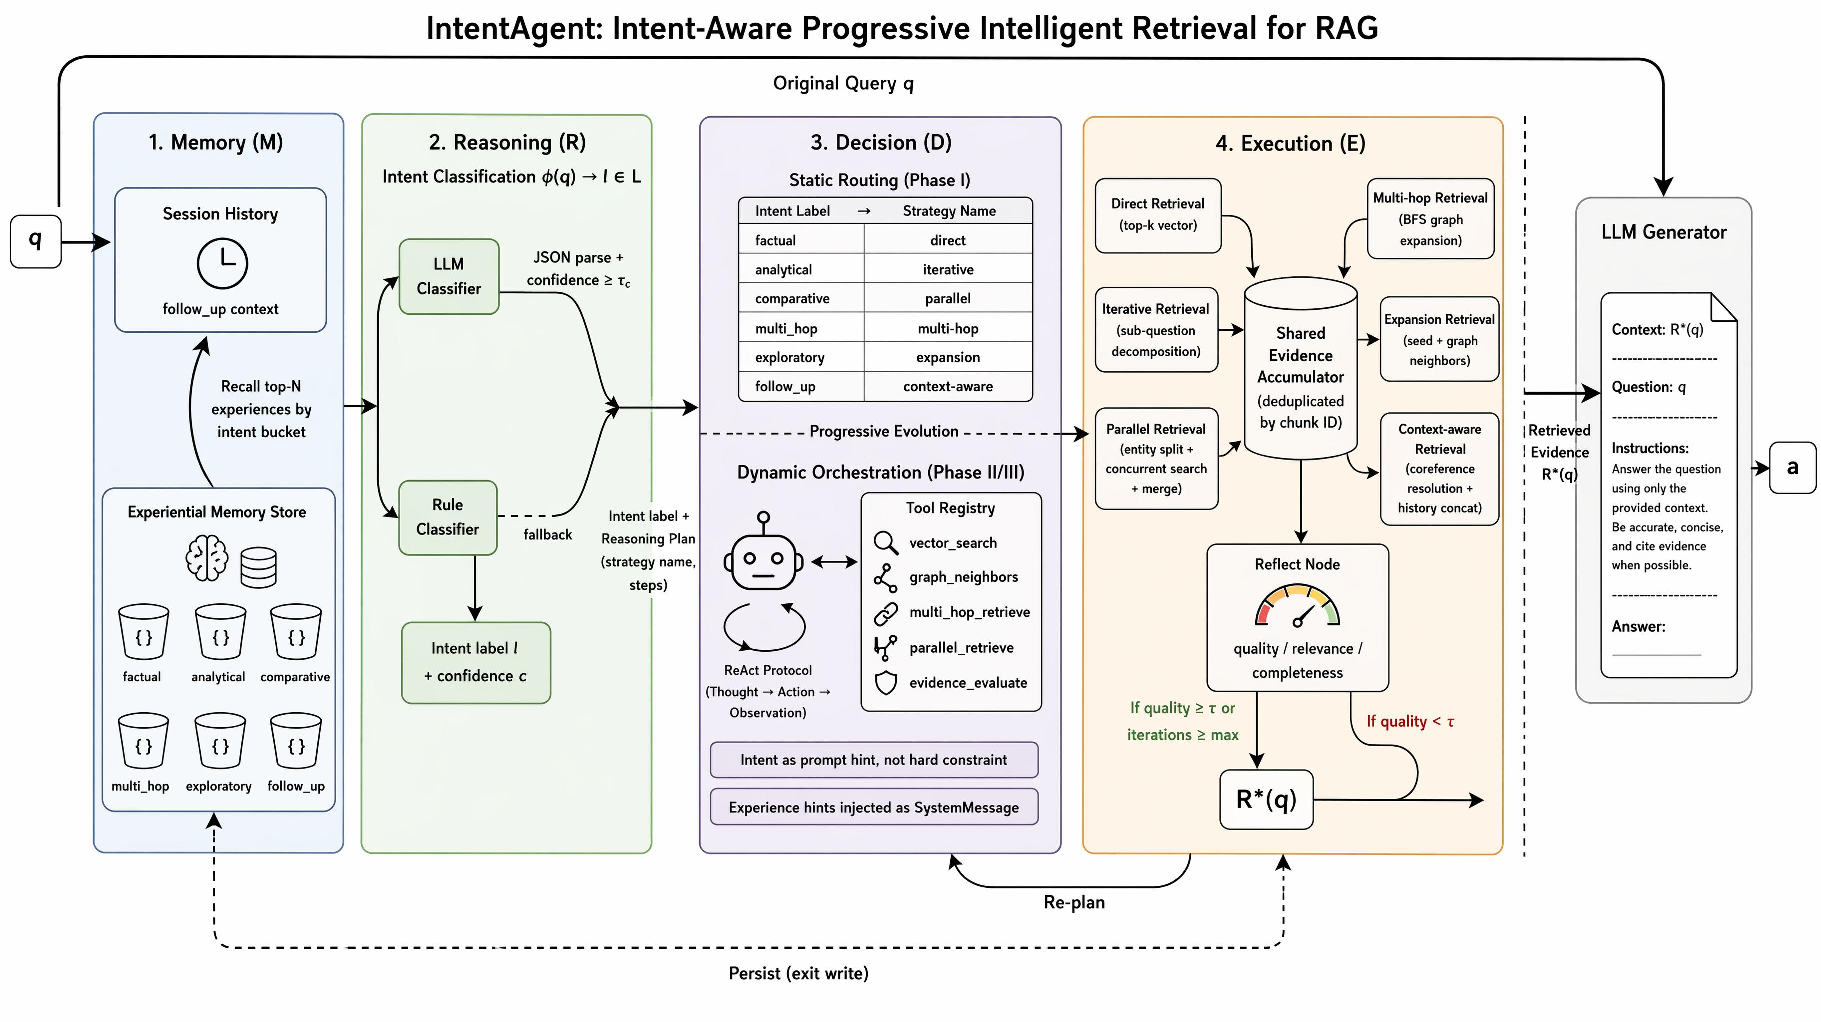
\includegraphics[width=\textwidth]{figures/figure2.pdf}
\caption{Overall architecture of IntentAgent. The system follows an M-R-D-E pipeline: Memory reads session history and experience memory; Reasoning identifies one of six query intents via the dual-path classifier; Decision switches between static mapping (Stage~1) and state-graph-based dynamic orchestration (Stages~2/3); Execution runs differentiated retrieval strategies with reflection-based quality gating. The three stages are color-coded.}
\label{fig:architecture}
\end{figure*}

IntentAgent follows a Memory $\to$ Reasoning $\to$ Decision $\to$ Execution (M-R-D-E) pipeline, implemented as a registry-driven pluggable architecture.

The Memory stage reads session history (when a session identifier exists) and injects multi-turn dialogue context into subsequent processing. In Stage~3, it additionally recalls same-intent historical experience entries from the experience store. The Reasoning stage runs the intent classifier $\phi(q)$ to produce an intent label $l$ and a confidence score $c$, then packages the result together with the query text into a reasoning plan containing the intent label, recommended strategy name, and execution step description. The Decision stage maps the reasoning plan to a concrete retrieval strategy instance: a deterministic lookup table in Stage~1, or an LLM-driven tool selection loop in Stages~2/3. The Execution stage runs the selected strategy, collects evidence passages and knowledge graph triples, optionally applies reranking and reflection-based evaluation, and returns the final retrieval results.

Pluggability is achieved through a registry mechanism in which each component is registered via decorators and the active implementation is specified at runtime through a configuration file. Switching between stages requires changing only a single configuration entry.

\subsection{Stage 1: Static Intent Routing}

\subsubsection{Dual-Path Classifier.}

The intent classifier adopts a cascaded design with an LLM-first path and a rule-based fallback. Formally, the classification function $\phi(q)$ is:
\begin{equation}
    \phi(q) = \begin{cases}
    (l_{\text{llm}}, c_{\text{llm}}) & \text{if } c_{\text{llm}} \geq \tau_c \wedge l_{\text{llm}} \in \mathcal{L} \\
    \phi_{\text{rule}}(q) & \text{otherwise}
    \end{cases}
\end{equation}
where $l_{\text{llm}}, c_{\text{llm}} = \text{LLM}(q)$ are the intent label and confidence returned by the LLM, $\tau_c = 0.6$ is the confidence threshold, and $\mathcal{L}$ is the valid label set.

The primary path sends a structured prompt to the LLM requesting a JSON-formatted classification result. The output undergoes strict parsing and validation: (1)~JSON parsing is attempted, with fallback to fenced extraction and greedy slicing upon failure; (2)~the label is verified to belong to $\mathcal{L}$; (3)~the confidence is checked against $\tau_c$. Failure at any step triggers the rule path.

The rule path $\phi_{\text{rule}}$ is a priority-ordered cascade of regular expressions $\{(r_i, l_i, c_i)\}_{i=1}^{M}$, where $r_i$ is a regex pattern, $l_i$ is the corresponding label, and $c_i$ is a fixed confidence:
\begin{equation}
    \phi_{\text{rule}}(q) = (l_j, c_j), \quad j = \min\{i \mid r_i \text{ matches } q\}
\end{equation}
If no rule matches, the default $(\texttt{factual}, 0.4)$ is returned. The LLM path captures semantically subtle intents, while the rule path guarantees continued operation when the LLM service is unavailable or produces unreliable outputs.

\subsubsection{Deterministic Intent-Strategy Mapping.}

The intent label is mapped to a retrieval strategy through a deterministic function $\mathcal{M}: \mathcal{L} \to \mathcal{S}$:
\begin{equation}
    \mathcal{M}(l) = \begin{cases}
    s_{\text{direct}} & l = \texttt{factual} \\
    s_{\text{iterative}} & l = \texttt{analytical} \\
    s_{\text{parallel}} & l = \texttt{comparative} \\
    s_{\text{multi\_hop}} & l = \texttt{multi\_hop} \\
    s_{\text{expansion}} & l = \texttt{exploratory} \\
    s_{\text{context}} & l = \texttt{follow\_up}
    \end{cases}
\end{equation}
Here $s_{\text{direct}}$ performs top-$k$ vector retrieval; $s_{\text{iterative}}$ decomposes the query into sub-questions and retrieves iteratively; $s_{\text{parallel}}$ splits the query into sub-queries $\{q_1, \ldots, q_m\}$ via regex, executes concurrent retrieval, and merges the results; $s_{\text{multi\_hop}}$ performs $h$-hop (default $h=2$) BFS graph expansion from seed retrieval results; $s_{\text{expansion}}$ adds additional neighbor exploration beyond the baseline hop count; and $s_{\text{context}}$ concatenates the most recent $H$ turns (default $H=3$) of session history for coreference resolution. All strategies conform to a unified interface $s: (q, \mathcal{K}, \mathcal{G}) \to \mathcal{R}$.

\subsubsection{End-to-End Flow.}

Given query $q$ and session identifier $\text{sid}$, the static routing pipeline is:
\begin{equation}
    \begin{aligned}
    \mathbf{h} &= \text{Memory}(\text{sid}) \\
    (l, c) &= \phi(q) \\
    s^* &= \mathcal{M}(l) \\
    \mathcal{R}(q) &= s^*(q, \mathcal{K}, \mathcal{G}) \\
    \mathcal{R}'(q) &= \text{Rerank}(q, \mathcal{R}(q))
    \end{aligned}
\end{equation}
where the reranking function scores results by Jaccard word-level overlap:
\begin{equation}
    \text{Rerank}(q, \mathcal{R}) = \text{sort}\!\left(\mathcal{R},\ \text{key}(c) = \frac{|W_q \cap W_c|}{|W_q \cup W_c|}\right)
\end{equation}
The intent label $l$, confidence $c$, and strategy name are recorded in the result metadata.

\subsection{Stage 2: Dynamic Tool Orchestration}

\subsubsection{Motivation.}

Static routing has three principal limitations: (1)~cross-intent blindness, whereby a query involving multiple intent types cannot be adequately served by a single strategy; (2)~absence of runtime feedback, whereby execution proceeds without adjustment even when retrieval quality is poor; and (3)~combinatorial explosion, whereby manually authoring hybrid strategies for all intent combinations leads to an exponential number of strategies.

Dynamic orchestration reframes strategy selection as a tool selection problem: each retrieval capability is encapsulated as an independent tool, and an LLM-based agent decides at runtime which tools to invoke and in what order.

\subsubsection{Tool Encapsulation.}

The existing retrieval primitives are encapsulated into five structured tools $\mathcal{T} = \{t_1, t_2, t_3, t_4, t_5\}$ following the principle of thin wrapping with zero new retrieval logic. Each tool $t_i: \Theta_i \to \mathcal{R}_i$ maps from a parameter space $\Theta_i$ to a retrieval result. Tool $t_1$ (vector retrieval) computes $t_1(q, k) = \text{top-}k\text{ nearest}(\text{embed}(q), \mathcal{K})$, returning the $k$ most semantically similar passages. Tool $t_2$ (graph neighbor expansion) returns $h$-hop neighbor triples $t_2(e, h) = \{(s, p, o) \in \mathcal{E} \mid \text{dist}(e, s) \leq h \vee \text{dist}(e, o) \leq h\}$ of entity $e$. Tool $t_3$ (multi-hop retrieval) combines seed retrieval with graph expansion: $t_3(q) = t_1(q, k) \cup t_2(\text{entities}(t_1(q, k)), h)$. Tool $t_4$ (parallel retrieval) executes $t_4(q) = \bigcup_{i=1}^{m} t_1(q_i, k)$ over sub-queries $\{q_i\}$. Tool $t_5$ (evidence evaluation) assesses the quality of collected evidence: $t_5(q, \mathcal{C}) \to (Q_{\text{quality}}, Q_{\text{relevance}}, Q_{\text{completeness}}) \in [0,1]^3$.

Cross-tool evidence accumulation is mediated by a shared tool context $\mathcal{C}$ that maintains a mapping $\mathcal{C}: \text{chunk\_id} \to \text{score}$. Each tool invocation updates this context as:
\begin{equation}
    \mathcal{C}[c.\text{id}] \leftarrow \max(\mathcal{C}[c.\text{id}],\ \text{score}(c)), \quad \forall c \in t_i(\theta_i)
\end{equation}
Deduplication retains the highest score per chunk. The merged output is $\text{merge}(\mathcal{C}) = \text{sort\_desc}(\mathcal{C})[:k]$.

\subsubsection{Agent Workflow over a Directed State Graph.}

\begin{figure}[htbp]
\centering
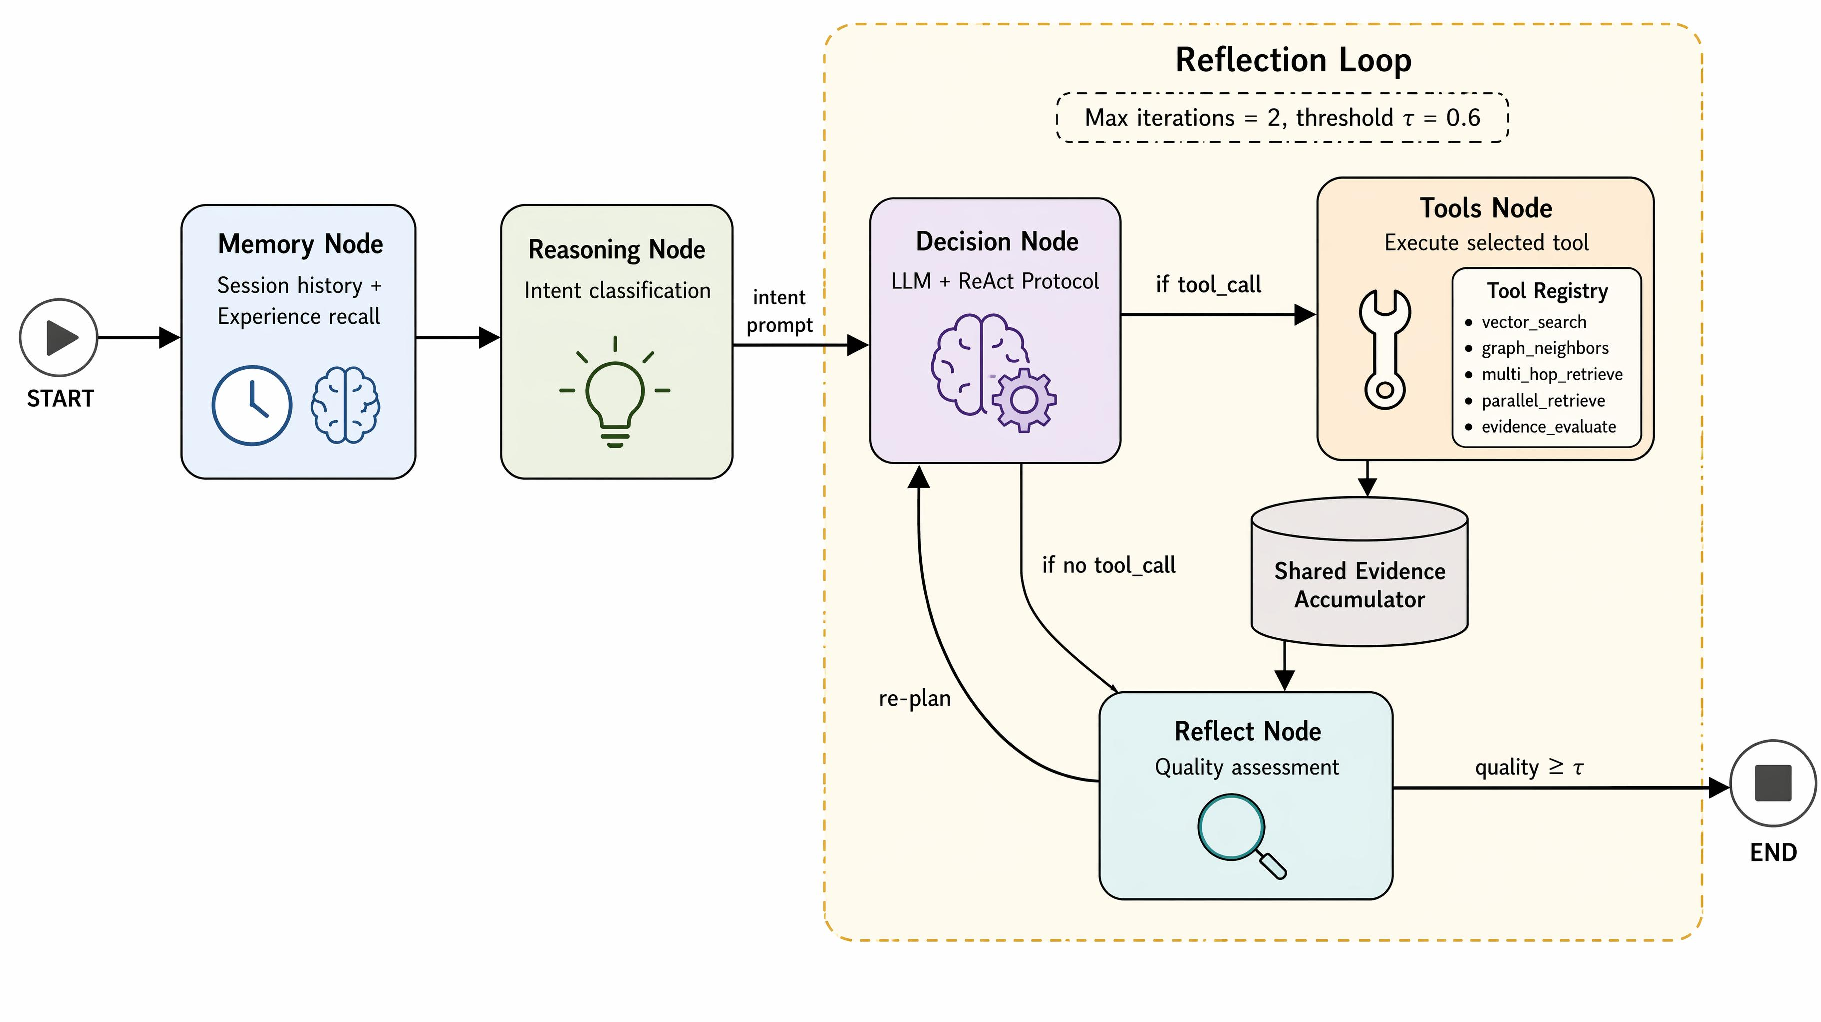
\includegraphics[width=\columnwidth]{figures/figure3.pdf}
\caption{Directed state graph topology. Five nodes (memory, reasoning, decision, tools, reflect) form a reflection loop via two conditional edges: the decision node routes to tools or reflect based on the LLM output; the reflect node triggers replanning back to the decision node when the quality score is below the threshold, thereby achieving closed-loop retrieval quality correction.}
\label{fig:state_graph}
\end{figure}

The retrieval process is modeled as a cyclic directed state graph $G_s = (V_s, E_s)$ with five nodes $V_s = \{v_{\text{mem}}, v_{\text{reas}}, v_{\text{dec}}, v_{\text{tool}}, v_{\text{ref}}\}$ and two conditional edges. The agent state is defined as the tuple $\mathbf{S} = (q, l, \mathbf{m}, n, Q, \mathbf{T}_{\log})$, comprising the query $q$, intent label $l$, message sequence $\mathbf{m}$, iteration count $n$, quality score $Q$, and tool invocation log $\mathbf{T}_{\log}$. The topology is $\text{START} \to v_{\text{mem}} \to v_{\text{reas}} \to v_{\text{dec}} \rightleftharpoons v_{\text{tool}} \rightleftharpoons v_{\text{ref}} \to \text{END}$.

The memory node $v_{\text{mem}}$ reads session history $\mathbf{h} = \text{Memory}(\text{sid})$, updates $\mathbf{m} \leftarrow \mathbf{m} \oplus \mathbf{h} \oplus [q]$, and initializes $n \leftarrow 0$. The reasoning node $v_{\text{reas}}$ invokes the intent classifier $l, c = \phi(q)$ and injects the label as a system message hint $\mathbf{m} \leftarrow \mathbf{m} \oplus [\text{``intent: } l \text{, conf: } c\text{''}]$; the intent serves as a hint rather than a hard constraint, thereby preserving the flexibility of the LLM across intent boundaries. The decision node $v_{\text{dec}}$ invokes the LLM bound with $\mathcal{T}$ to produce $a = \text{LLM}_{\mathcal{T}}(\mathbf{m})$, where $a \in \{(\text{tool\_call}, t_i, \theta_i)\} \cup \{\text{final\_answer}\}$. The tools node $v_{\text{tool}}$ executes $r_i = t_i(\theta_i)$, accumulates $\mathcal{C} \leftarrow \mathcal{C} \cup r_i$, and logs $\mathbf{T}_{\log} \leftarrow \mathbf{T}_{\log} \oplus [t_i]$. The reflect node $v_{\text{ref}}$ computes $Q = \text{Eval}(q, \text{merge}(\mathcal{C}))$ and increments $n \leftarrow n + 1$.

The routing functions for the two conditional edges are:
\begin{equation}
    \text{route}_1(a) = \begin{cases}
    v_{\text{tool}} & \text{if } a = (\text{tool\_call}, t_i, \theta_i) \\
    v_{\text{ref}} & \text{otherwise}
    \end{cases}
\end{equation}
\begin{equation}
    \text{route}_2(Q, n) = \begin{cases}
    \text{END} & \text{if } Q \geq \tau \vee n \geq n_{\max} \\
    v_{\text{dec}} & \text{otherwise}
    \end{cases}
\end{equation}
where $\tau = 0.6$ is the quality threshold and $n_{\max} = 2$ is the maximum iteration count.

\subsubsection{Reasoning-Action Protocol Adapter.}

A protocol adapter wraps the generic LLM abstraction into a compatible chat model by formatting the message list into the reasoning-action text protocol (Thought: \ldots\ Action: \ldots\ Action Input: \ldots) and parsing tool invocation requests into structured objects. The output space of the LLM at each decision step is:
\begin{equation}
    \text{LLM}_{\mathcal{T}}(\mathbf{m}) \to \begin{cases}
    (\text{Action}: t_i,\ \text{Input}: \theta_i) & \text{continue retrieval} \\
    (\text{Final Answer}: a) & \text{terminate}
    \end{cases}
\end{equation}
The parser employs priority-based regex matching: when both Final Answer and Action patterns appear, the earlier one takes precedence; when only Action is present, JSON parameters are parsed via greedy brace matching; when neither is found, the raw output is returned as the final answer. This design decouples IntentAgent from provider-specific function calling interfaces, enabling any text-completion LLM to drive tool selection.

The quality evaluation function $\text{Eval}(q, a)$ in $v_{\text{ref}}$ fuses multiple heuristic signals. Let $W_q$ and $W_a$ denote the token sets of the query and answer, $L = |a.\text{text}|$ the answer length, and $E = a.\text{evidence\_ids}$ the evidence set:
\begin{equation}
    Q_{\text{overlap}} = \frac{|W_q \cap W_a|}{\max(1, |W_q|)}, \quad Q_{\text{evidence}} = \begin{cases} 1.0 & |E| > 0 \\ 0.5 & |E| = 0 \end{cases}
\end{equation}
\begin{equation}
    Q_{\text{relevance}} = 0.5 \cdot Q_{\text{overlap}} + 0.5 \cdot Q_{\text{evidence}}
\end{equation}
\begin{equation}
    Q_{\text{completeness}} = \min\!\left(1,\ \frac{L}{4 \cdot L_{\min}}\right)
\end{equation}
\begin{equation}
    Q_{\text{quality}} = 0.5 \cdot Q_{\text{relevance}} + 0.5 \cdot Q_{\text{completeness}}
\end{equation}
where $L_{\min}$ is the minimum answer length parameter. If a refusal pattern (e.g., ``I do not know'') is detected, $Q_{\text{quality}} = 0.2$ is returned to trigger replanning.

\subsection{Stage 3: Experience Memory Augmentation}

\subsubsection{Motivation: From Stateless to Stateful.}

Although Stage~2 grants the LLM autonomy in tool selection, every decision starts from scratch. Even after the system has successfully handled numerous same-intent queries, the accumulated experience is lost when the session ends. Experience memory augmentation draws on the behavioral pattern of human experts, who select strategies based on experience with similar past problems rather than exploring anew each time.

\subsubsection{Experience Entry Data Model.}

Each experience record is defined as the tuple $e = (l, q, \mathbf{T}_{\text{seq}}, n, Q_f, o, \lambda, a, \mathbf{E}, h, \text{ts})$, comprising the intent label $l$ (bucket key), query text $q$, tool invocation sequence $\mathbf{T}_{\text{seq}}$, reflection iteration count $n$, final quality score $Q_f$, outcome class $o \in \{\text{success}, \text{lesson}\}$, avoidance note $\lambda$, answer text $a$, evidence chunk IDs $\mathbf{E}$, hit count $h$, and timestamp $\text{ts}$.

Entries are classified by comparing $Q_f$ against the threshold $\tau$:
\begin{equation}
    o = \begin{cases}
    \text{success} & \text{if } Q_f \geq \tau \quad \text{(full tool sequence and answer retained)} \\
    \text{lesson} & \text{if } Q_f < \tau \quad \text{(tool sequence and avoidance note only, } a \leftarrow \varnothing\text{)}
    \end{cases}
\end{equation}
Lessons discard low-quality answers to prevent error propagation.

\subsubsection{Three-Phase Closed Loop.}

The experience memory lifecycle follows a recall-inject-persist closed loop.

In the recall phase, before a query enters the state graph, the intent classifier produces $l = \phi(q).\text{label}$, which serves as the key to retrieve the top-$N_r$ (default $N_r = 3$) same-intent entries from the store $\mathcal{B}_l$:\begin{equation}
    \text{Recall}(l, N_r) = \text{top}_{N_r}\!\left(\mathcal{B}_l,\ \text{key} = (Q_f \downarrow,\ h \downarrow)\right)
\end{equation}

In the inject phase, recalled entries are rendered as a structured system message $\mathbf{m}_{\text{exp}}$ and prepended to the initial state: $\mathbf{m} \leftarrow [\mathbf{m}_{\text{exp}}] \oplus \mathbf{m}$. Experiences are injected as hints rather than as constraints, so that the LLM retains full decision autonomy and outdated experiences do not mislead the agent in novel scenarios.

In the persist phase, after query completion, a new entry $e_{\text{new}}$ is distilled from the final state and written to storage: $\mathcal{B}_l \leftarrow \mathcal{B}_l \cup \{e_{\text{new}}\}$. If an existing entry $e_{\text{old}}$ shares the deduplication key $(\mathbf{T}_{\text{seq}}, o)$, a merge update is performed:
\begin{equation}
    e_{\text{old}}.Q_f \leftarrow \max(e_{\text{old}}.Q_f,\ e_{\text{new}}.Q_f), \quad e_{\text{old}}.h \leftarrow e_{\text{old}}.h + 1
\end{equation}

\subsubsection{Persistent Storage Design.}

The experience store employs disk-based intent bucketing. Each intent label $l \in \mathcal{L}$ corresponds to an independent JSONL file $\mathcal{B}_l$, ensuring write atomicity and crash recoverability. Deduplication uses the key $\kappa(e) = (\mathbf{T}_{\text{seq}}, o)$; entries sharing the same key undergo merge updates. Each bucket has a capacity limit $C_{\max}$ (default 200); when $|\mathcal{B}_l| > C_{\max}$, a cold-old-first eviction policy is applied:
\begin{equation}
    \mathcal{B}_l \leftarrow \text{top}_{C_{\max}}\!\left(\mathcal{B}_l,\ \text{key} = (h \downarrow,\ \text{ts} \downarrow)\right)
\end{equation}
Because experiences are bucketed by intent, recall reads only a single small file, with time complexity $O(|\mathcal{B}_l| \log N_r)$.


\section{Experiments}

\subsection{Experimental Setup}

\subsubsection{Datasets.}

We evaluate IntentAgent on three widely used multi-hop question answering benchmarks. HotpotQA~\cite{ref20} contains approximately 113K questions that require reasoning across two Wikipedia paragraphs, covering both bridge reasoning and comparison reasoning; we use the development set under the distractor setting. 2WikiMultiHopQA~\cite{ref21} is a multi-hop QA dataset constructed from Wikipedia and Wikidata with reasoning chain annotations, covering comparison, inference, composition, and bridge reasoning types. MuSiQue~\cite{ref22} is a controllably constructed multi-hop QA dataset that generates 2--4 hop composite questions by combining single-hop questions, presenting higher reasoning difficulty; we evaluate on both the answerable subset (MuSiQue-Ans) and the full subset (MuSiQue-Full).

For each dataset, we randomly sample 500 questions (seed = 42) to balance evaluation coverage and computational cost.

\subsubsection{Evaluation Metrics.}

We adopt two standard QA evaluation metrics: Exact Match (EM), which checks whether the normalized prediction exactly matches the reference answer, and token-level F1, defined as the harmonic mean of token-level precision and recall between the prediction and the reference.

\subsubsection{Backbone Models and Configuration.}

To verify generalization across LLM scales, we select two backbone models: Qwen3-8B (8 billion parameters) and Qwen3-32B (32 billion parameters). All backbones are used uniformly for intent classification, retrieval-stage reasoning, and final answer generation. The temperature is set to 0 for reproducibility. The embedding model is text-embedding-3-small throughout. Retrieval parameters are: top-$k$ = 5, multi-hop hops $h$ = 2, reflection quality threshold $\tau$ = 0.6, and maximum reflection rounds $n_{\max}$ = 2.

\subsubsection{Baselines.}

We compare IntentAgent against three categories of representative methods. Text retrieval methods include Vanilla RAG (standard vector retrieval followed by generation) and RAPTOR~\cite{ref23} (hierarchical retrieval tree). Graph-augmented retrieval methods include TOG~\cite{ref24} (knowledge graph reasoning navigation) and G-Retriever~\cite{ref25} (graph neural network joint retrieval). Hybrid retrieval methods include LightRAG~\cite{ref26} (dual-level retrieval), GraphRAG~\cite{ref27} (community summarization), and HippoRAG~\cite{ref28} (hippocampal memory indexing). We also report an LLM-only baseline (without retrieval) for each backbone to quantify the marginal benefit of retrieval augmentation.

\subsection{Main Results}

Table~\ref{tab:main_results} reports results under both Qwen3-8B and Qwen3-32B backbones.

\begin{table}[htbp]
\centering
\caption{Main results under Qwen3-8B and Qwen3-32B backbones. Best values are in bold.}
\label{tab:main_results}
\resizebox{\textwidth}{!}{
\begin{tabular}{ll|cc|cc|cc|cc}
\toprule
\textbf{Type} & \textbf{Method} & \textbf{2Wiki EM} & \textbf{2Wiki F1} & \textbf{HotpotQA EM} & \textbf{HotpotQA F1} & \textbf{MuSiQue-A EM} & \textbf{MuSiQue-A F1} & \textbf{MuSiQue-F EM} & \textbf{MuSiQue-F F1} \\
\midrule
\multicolumn{10}{c}{\textit{Backbone: Qwen3-8B}} \\
\midrule
LLM only & Qwen3-8B & 0.270 & 0.300 & 0.222 & 0.306 & 0.050 & 0.134 & 0.064 & 0.128 \\
\midrule
Text & Vanilla RAG & 0.231 & 0.283 & 0.341 & 0.428 & 0.113 & 0.156 & 0.058 & 0.105 \\
Text & RAPTOR & 0.428 & 0.464 & 0.382 & 0.547 & 0.205 & 0.318 & \textbf{0.171} & 0.215 \\
\midrule
Graph & TOG & 0.265 & 0.324 & 0.189 & 0.211 & 0.062 & 0.087 & 0.055 & 0.059 \\
Graph & G-Retriever & 0.357 & 0.395 & 0.308 & 0.439 & 0.156 & 0.214 & 0.082 & 0.118 \\
\midrule
Hybrid & LightRAG & 0.301 & 0.319 & 0.342 & 0.412 & 0.121 & 0.142 & 0.078 & 0.146 \\
Hybrid & GraphRAG & 0.314 & 0.327 & 0.371 & 0.498 & 0.169 & 0.295 & 0.137 & 0.158 \\
Hybrid & HippoRAG & 0.535 & 0.638 & 0.451 & 0.554 & 0.241 & 0.305 & 0.162 & \textbf{0.258} \\
\midrule
Proposed & \textbf{IntentAgent} & \textbf{0.551} & \textbf{0.654} & \textbf{0.462} & \textbf{0.571} & \textbf{0.249} & \textbf{0.321} & 0.155 & 0.247 \\
\midrule
\midrule
\multicolumn{10}{c}{\textit{Backbone: Qwen3-32B}} \\
\midrule
LLM only & Qwen3-32B & 0.322 & 0.375 & 0.260 & 0.380 & 0.064 & 0.172 & 0.082 & 0.156 \\
\midrule
Text & Vanilla RAG & 0.253 & 0.316 & 0.383 & 0.456 & 0.136 & 0.184 & 0.056 & 0.115 \\
Text & RAPTOR & 0.471 & 0.537 & 0.422 & 0.619 & 0.227 & \textbf{0.358} & 0.186 & 0.247 \\
\midrule
Graph & TOG & 0.312 & 0.363 & 0.225 & 0.234 & 0.063 & 0.100 & 0.058 & 0.068 \\
Graph & G-Retriever & 0.394 & 0.457 & 0.343 & 0.516 & 0.176 & 0.239 & 0.094 & 0.139 \\
\midrule
Hybrid & LightRAG & 0.329 & 0.340 & 0.386 & 0.456 & 0.142 & 0.155 & 0.093 & 0.167 \\
Hybrid & GraphRAG & 0.368 & 0.369 & 0.407 & 0.569 & 0.197 & 0.348 & 0.145 & 0.174 \\
Hybrid & HippoRAG & 0.576 & 0.696 & 0.470 & 0.621 & 0.262 & 0.332 & \textbf{0.190} & \textbf{0.290} \\
\midrule
Proposed & \textbf{IntentAgent} & \textbf{0.589} & \textbf{0.712} & \textbf{0.483} & \textbf{0.638} & \textbf{0.271} & 0.345 & 0.182 & 0.279 \\
\bottomrule
\end{tabular}
}
\end{table}

\begin{figure}[htbp]
\centering
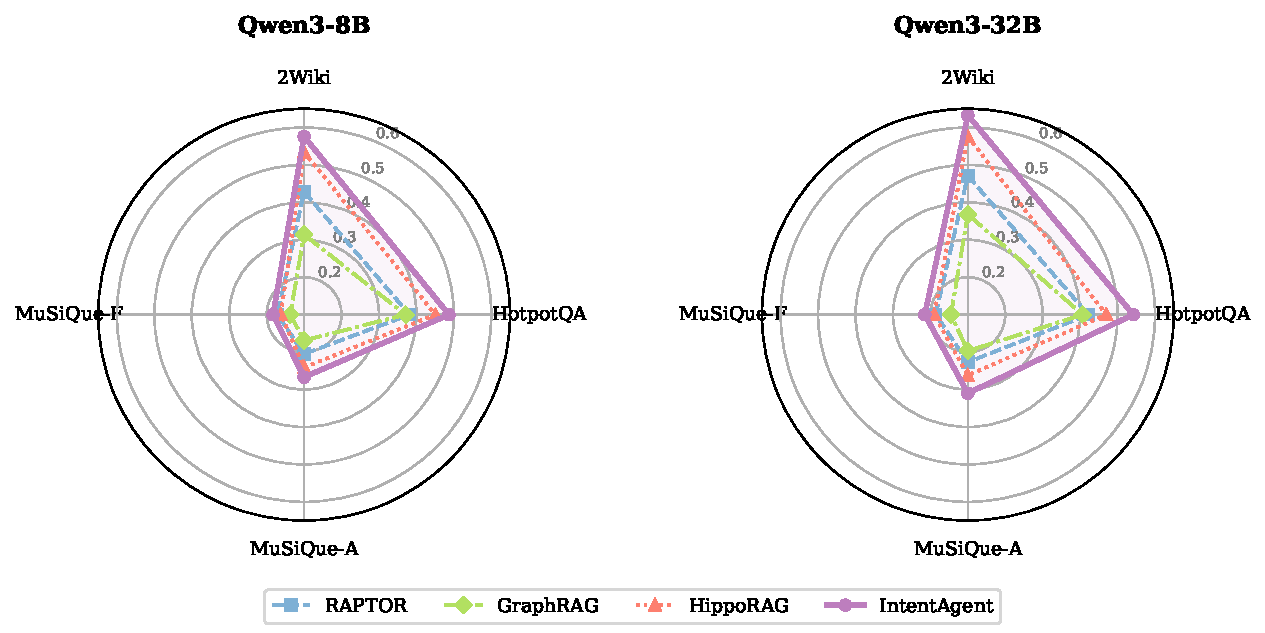
\includegraphics[width=\textwidth]{figures/fig4_radar.pdf}
\caption{EM performance profiles of IntentAgent and the top-3 baselines across four datasets (left: Qwen3-8B; right: Qwen3-32B). IntentAgent spans the largest area on most axes, with particularly pronounced advantages on 2WikiMultiHopQA and HotpotQA.}
\label{fig:radar}
\end{figure}

\subsection{Ablation Study}

To verify the contribution of each component, we design the following ablation variants: (1)~w/o Intent removes intent classification and routes all queries to direct retrieval; (2)~w/o Dynamic retains only static routing; (3)~w/o Reflect employs dynamic orchestration but removes the reflection node; (4)~w/o Memory disables experience memory; and (5)~w/o Dual-Path removes the rule-based fallback path and relies solely on the LLM classifier.

Table~\ref{tab:ablation} reports ablation results under the Qwen3-32B backbone.

\begin{table}[htbp]
\centering
\caption{Ablation results (backbone: Qwen3-32B).}
\label{tab:ablation}
\resizebox{\textwidth}{!}{
\begin{tabular}{l|cc|cc|cc|cc}
\toprule
\textbf{Variant} & \textbf{2Wiki EM} & \textbf{2Wiki F1} & \textbf{HotpotQA EM} & \textbf{HotpotQA F1} & \textbf{MuSiQue-A EM} & \textbf{MuSiQue-A F1} & \textbf{MuSiQue-F EM} & \textbf{MuSiQue-F F1} \\
\midrule
\textbf{IntentAgent (Full)} & \textbf{0.589} & \textbf{0.712} & \textbf{0.483} & \textbf{0.638} & \textbf{0.271} & \textbf{0.345} & \textbf{0.182} & \textbf{0.279} \\
w/o Intent & 0.513 & 0.599 & 0.434 & 0.573 & 0.226 & 0.291 & 0.145 & 0.248 \\
w/o Dynamic & 0.528 & 0.661 & 0.455 & 0.573 & 0.255 & 0.301 & 0.172 & 0.264 \\
w/o Reflect & 0.562 & 0.669 & 0.466 & 0.615 & 0.254 & 0.319 & 0.165 & 0.256 \\
w/o Memory & 0.568 & 0.677 & 0.463 & 0.617 & 0.258 & 0.326 & 0.179 & 0.270 \\
w/o Dual-Path & 0.582 & 0.679 & 0.463 & 0.615 & 0.265 & 0.336 & 0.179 & 0.266 \\
\bottomrule
\end{tabular}
}
\end{table}

\begin{figure}[htbp]
\centering
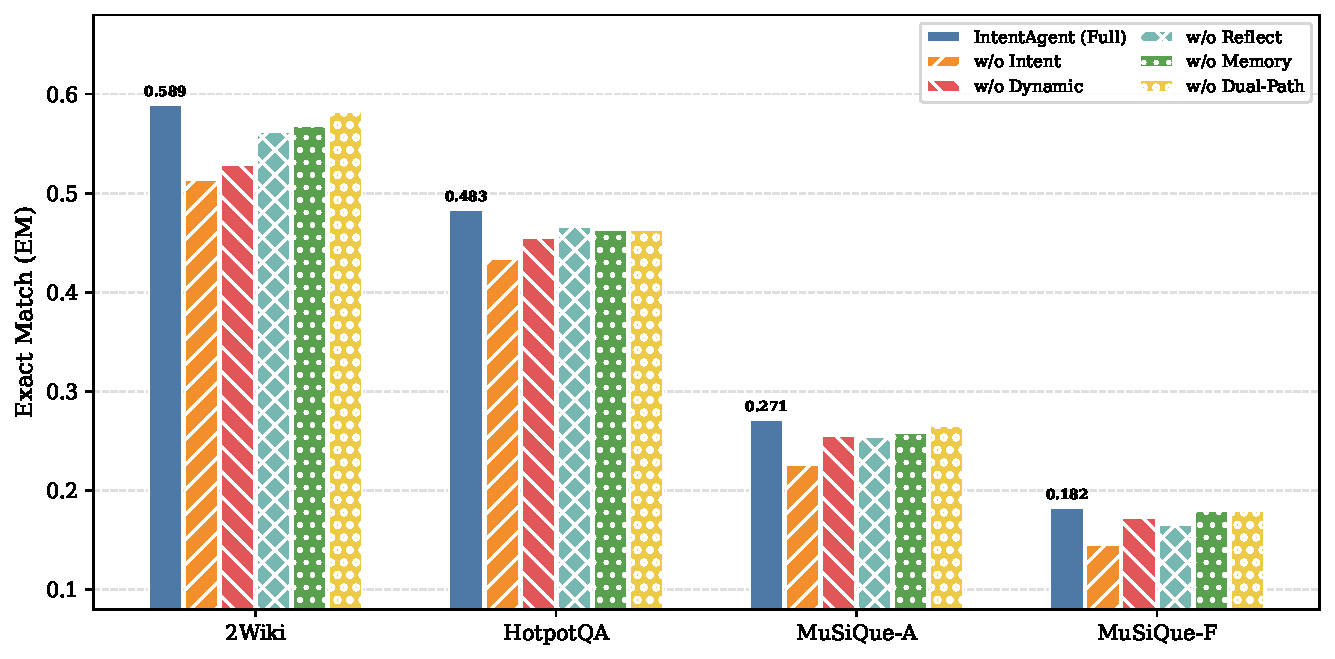
\includegraphics[width=\textwidth]{figures/fig5_ablation.pdf}
\caption{Ablation results (backbone: Qwen3-32B). EM comparison across four datasets. Removing intent classification (w/o Intent) causes the largest performance drop, confirming that intent awareness constitutes the primary contribution.}
\label{fig:ablation}
\end{figure}

\subsection{Further Analysis}

\subsubsection{Retrieval Quality Analysis.}

To understand differences at the retrieval stage, we report average evidence coverage (the proportion of retrieved results that contain evidence passages needed to support the answer) and average relevance score (semantic relevance between retrieval results and the query, evaluated by the LLM on a 1--5 scale).

\begin{table}[htbp]
\centering
\caption{Retrieval quality analysis (backbone: Qwen3-32B, HotpotQA).}
\label{tab:retrieval_quality}
\begin{tabular}{l|cc}
\toprule
\textbf{Method} & \textbf{Evidence Coverage} & \textbf{Avg. Relevance} \\
\midrule
Vanilla RAG & 0.414 & 2.90 \\
RAPTOR & 0.555 & 3.67 \\
TOG & 0.304 & 2.49 \\
G-Retriever & 0.520 & 3.30 \\
LightRAG & 0.445 & 3.21 \\
GraphRAG & 0.507 & 3.59 \\
HippoRAG & 0.635 & 3.77 \\
\midrule
IntentAgent (static) & 0.554 & 3.61 \\
IntentAgent (dynamic) & 0.700 & 4.01 \\
IntentAgent (memory) & \textbf{0.738} & \textbf{4.26} \\
\bottomrule
\end{tabular}
\end{table}

\subsubsection{Scale Sensitivity Analysis.}

To verify stability across evaluation scales, we evaluate IntentAgent and the principal baselines on HotpotQA at sample sizes of 100, 200, 300, 400, and 500.

\begin{table}[htbp]
\centering
\caption{Scale sensitivity: EM at different sample sizes (backbone: Qwen3-32B, HotpotQA).}
\label{tab:scale_sensitivity}
\begin{tabular}{l|ccccc}
\toprule
\textbf{Method} & \textbf{N=100} & \textbf{N=200} & \textbf{N=300} & \textbf{N=400} & \textbf{N=500} \\
\midrule
RAPTOR & 0.393 & 0.433 & 0.430 & 0.423 & 0.422 \\
GraphRAG & 0.415 & 0.387 & 0.404 & 0.405 & 0.407 \\
HippoRAG & 0.493 & 0.458 & 0.470 & 0.459 & 0.470 \\
IntentAgent & \textbf{0.505} & \textbf{0.473} & \textbf{0.489} & \textbf{0.487} & \textbf{0.483} \\
\bottomrule
\end{tabular}
\end{table}

\subsubsection{Experience Memory Growth Curve.}

To verify the cumulative effect of experience memory, we process 500 queries sequentially in windows of 50 queries each and report the average EM and F1 of IntentAgent (with experience memory enabled) per window.

\begin{table}[htbp]
\centering
\caption{Experience memory growth curve: performance over accumulated queries (backbone: Qwen3-32B, HotpotQA).}
\label{tab:memory_growth}
\begin{tabular}{l|cc}
\toprule
\textbf{Query Window} & \textbf{EM} & \textbf{F1} \\
\midrule
1--50 (cold start) & 0.424 & 0.571 \\
51--100 & 0.455 & 0.602 \\
101--200 & 0.463 & 0.619 \\
201--300 & 0.474 & 0.638 \\
301--400 & 0.492 & 0.645 \\
401--500 & \textbf{0.495} & \textbf{0.647} \\
\bottomrule
\end{tabular}
\end{table}


\section{Analysis and Discussion}

\subsection{Necessity of Intent Awareness}

The performance drop in the w/o Intent variant provides the most direct evidence. After removing intent classification, all queries are uniformly routed to direct retrieval: multi-hop reasoning queries suffer substantially because graph expansion becomes unavailable, and comparative queries receive incomplete information because parallel retrieval is disabled.

This result validates the central proposition of this paper: queries of different intent types genuinely require differentiated retrieval strategies, and intent classification is not an optional optimization but rather a prerequisite for effective retrieval. From an efficiency perspective, the additional cost of intent classification (approximately one LLM call) is well justified by the resulting improvement in retrieval quality.

\subsection{Value of the Static-to-Dynamic Transition}

The gap between the w/o Dynamic variant and the full system reveals the incremental value of dynamic orchestration over static routing. This gap is more pronounced in two scenarios. First, real-world datasets contain mixed-intent queries (e.g., comparison questions in HotpotQA that combine comparison and bridging characteristics); static routing can assign only a single strategy, whereas dynamic orchestration allows the LLM to flexibly compose multiple tools. Second, static routing commits to a strategy without recourse, while the reflection node in dynamic orchestration can detect $Q < \tau$ after the initial retrieval round and trigger replanning. The performance gap of the w/o Reflect variant quantifies the contribution of the reflection loop.

\subsection{Cumulative Effect of Experience Memory}

The comparison with the w/o Memory variant quantifies the contribution of experience memory. This mechanism exhibits three cumulative effects. As same-intent queries accumulate, success paths and failure lessons gradually populate the store, and subsequent queries can directly reuse validated tool sequences, thereby converging from a cold start to a warm start. Success paths receive incrementing hit counts upon reuse and gain higher priority in recall ranking, creating a positive feedback loop. Failure lessons enable the LLM to skip tool sequences that have previously proven ineffective, thus avoiding repeated mistakes.

\subsection{Limitations}

This work has the following limitations. (1)~The six intent classes may not cover all query scenarios; types such as temporal reasoning and numerical computation are not included in the current taxonomy. (2)~LLM-based intent classification requires one additional call (approximately 200 tokens), which may be unacceptable in scenarios with extremely tight latency constraints. (3)~Experience entries may become stale as the knowledge base evolves; the current design does not incorporate a knowledge-base-version-aware expiration mechanism.


\section{Conclusion}

This paper proposes IntentAgent, an intent-aware progressive intelligent retrieval method for Retrieval-Augmented Generation. IntentAgent elevates query intent to a first-class citizen in retrieval strategy selection and strikes a balance between controllability and adaptivity through three-stage progressive evolution: static intent routing, dynamic tool orchestration, and experience memory augmentation.

Experiments on HotpotQA, 2WikiMultiHopQA, and MuSiQue under both Qwen3-8B and Qwen3-32B backbones demonstrate that intent-aware differentiated retrieval matches each query type to its most suitable retrieval path, achieving the best or highly competitive performance compared with existing text-based, graph-based, and hybrid retrieval methods. Ablation studies confirm the independent contribution of intent classification, dynamic orchestration, the reflection loop, and experience memory.

Future work will proceed in three directions: (1)~hierarchical intent classification with fine-grained subtypes to further optimize strategy matching; (2)~vector-based experience recall that moves beyond exact intent-label matching by leveraging query embeddings for semantic-level retrieval of similar experiences; and (3)~cross-modal extension of the intent-aware retrieval paradigm to multimodal RAG scenarios.

\bibliographystyle{splncs04}
\bibliography{references}

\end{document}
